\documentclass{article}[14pt, letterpaper, Times New Roman]
\usepackage{graphicx}
\graphicspath{ {images/} }
\usepackage{listings}
\usepackage{geometry}
\geometry{margin=1in}

\title{2P04 Lab 3}
\author{Talha Ahmad, 400517273}

\begin{document}

\maketitle

\section{Lecture 9}

\subsection{Lecture Question}

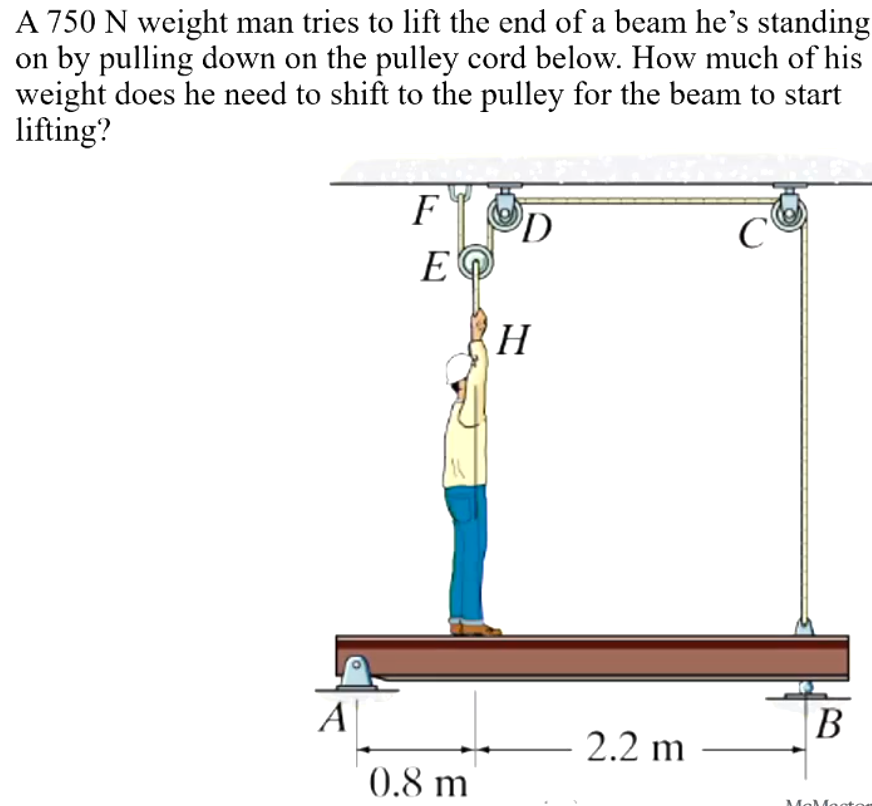
\includegraphics[width=15cm]{l9-lq.png}

We know that the system starts off with in equilibrium due to the reaction force at A from the man's weight and the reaction moment at A due to the torque from the man's weight.
We're asked to find when the net torque shifts in such a manner that a clockwise torque is produced instead.
We know that $HE = 2DH$.
Therefore, the tension in the rope pulling up the man is double the weight he's shifting to the pulley.

We can create the following equation for net torque:

\[ 3T - 0.8(750 - 2T) > 0 \]

We know that the tension the man transfers over is half his weight, so in order to see how much weight he loses from where he's standing we need to subtract double the tension.
Now we can go ahead and solve the above inequality to find the minimum tension required:

\[ 3T - 600 + 1.6T > 0 \]

\[ 4.6T > 600 \]

\[ T > 130.43 \]

Therefore, the weight that the man needs to transfer over in order to shift the net torque to a clockwise direction is 260.86 N.
This makes his current weight 489.14 N.

\subsection{Lecture Quiz}

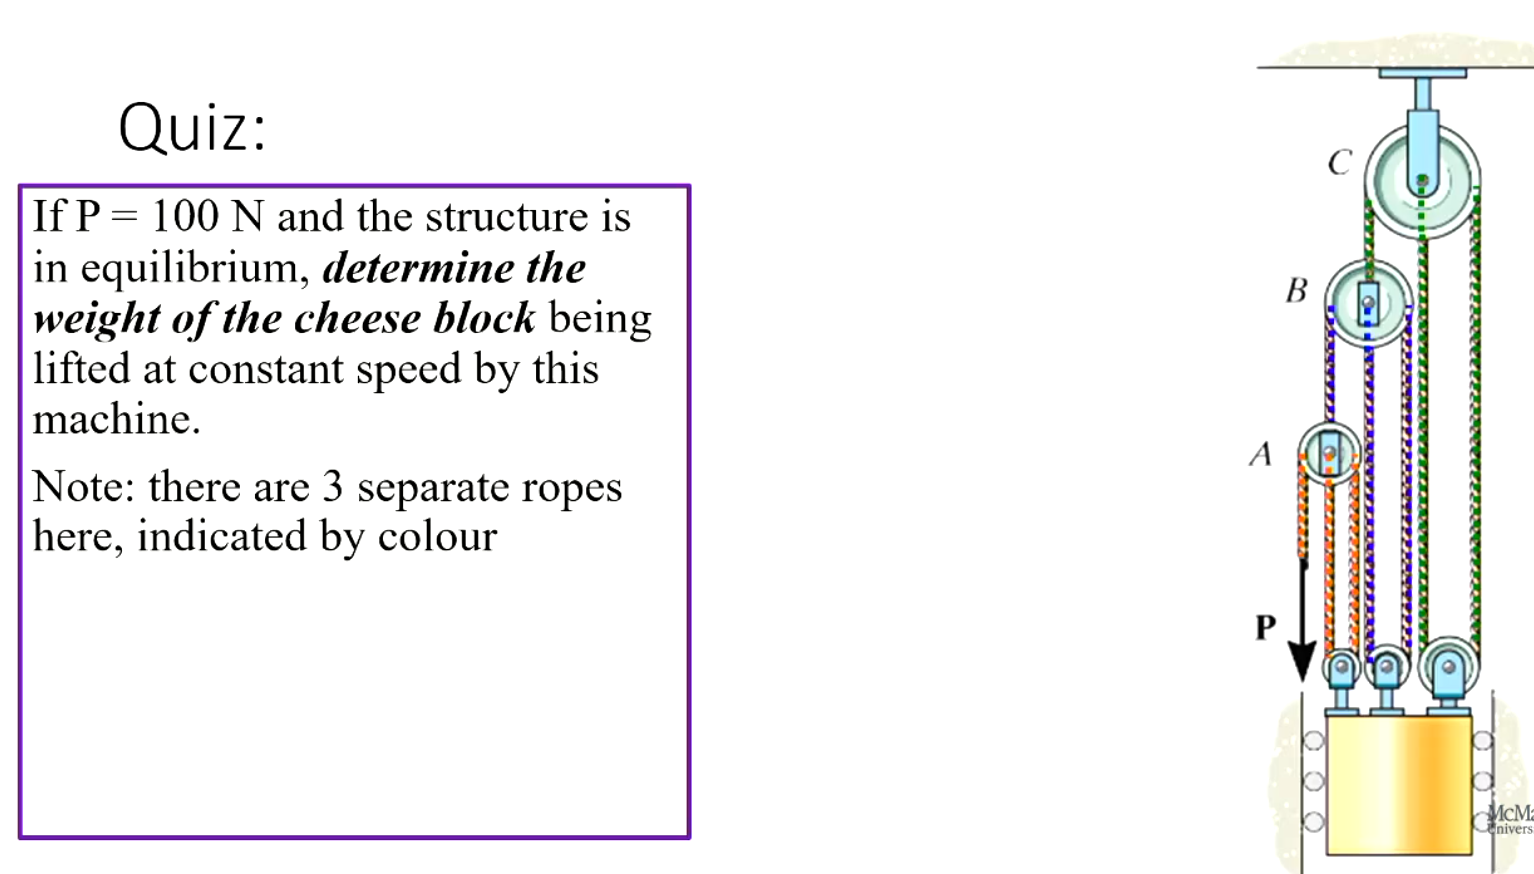
\includegraphics[width=15cm]{l9-quiz.png}

We know that the orange rope must be equal to P since the pulleys are assumed to be ideal without any friction.

We know that $3A = B$ since pulley A must be in equilibrium.

We know that $3B = C$ since pulley B must be in equilibrium.

And given how the ropes are connected to the cheese block, we know that $2A + 2B + 2C = cheese$.

If P = 100 N, then A = 100 N, B = 300 N, C = 900 N, and the cheese block weighs 2600 N.

\medskip

Reflection: In this lecture we were introduced to frames and machines and how we can solve for the forces and moments in them. We learned how to calculate the forces and moments in a system with multiple components. This is useful in real life applications where we have to deal with multiple components in a system. Moreover, we learned how to calculate the forces and moments in a system with multiple components.

\subsection{Problem Bank Question}

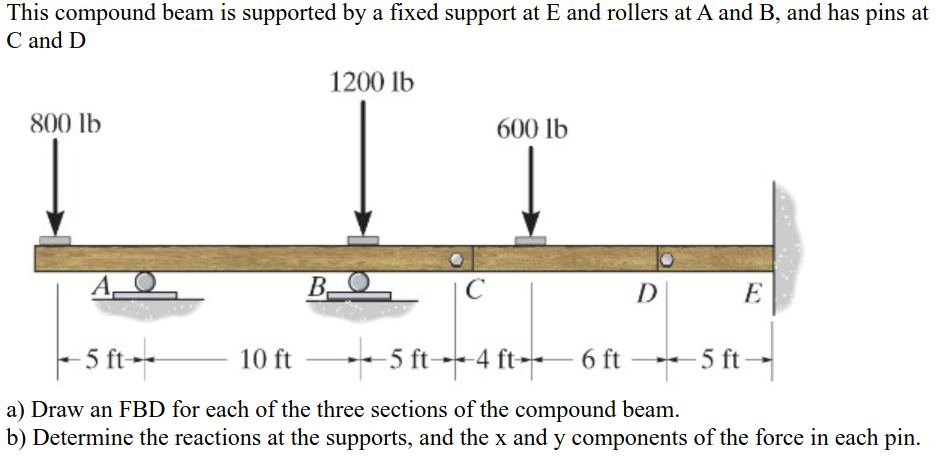
\includegraphics[width=15cm]{l9-pbq.png}

The FBD can be seen below:

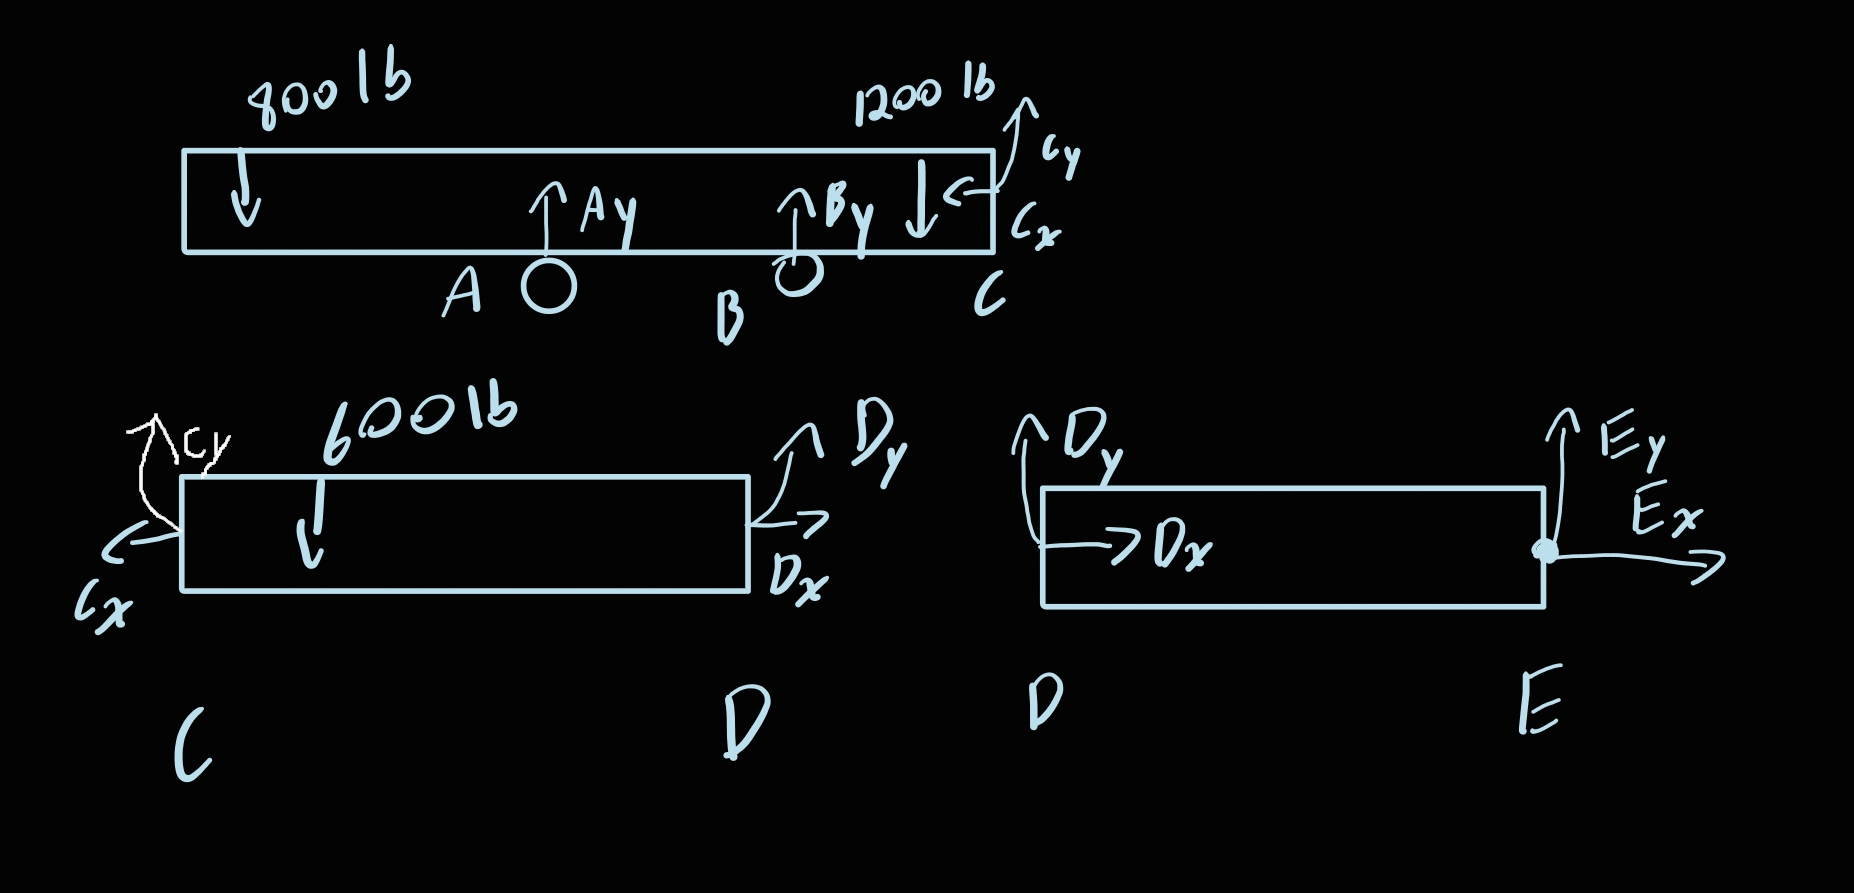
\includegraphics[width=15cm]{l9-pbq-fbd.png}

We can create equations for each of the sections and solve for the unknowns.

Maple code to solve:

\begin{lstlisting}[language=matlab]
restart: solve([
-800 + Ay + By - 1200 + Cy,
Cy-600+Dy,
Dy+Ey,
Cx,
Cx-Dx,
Dx+Ex,
800 * 5 - 1200*10 + 10*By + 15*Cy,
800*20 - 15*Ay - 5*By + 5*1200 - 600*4 + Dy*10
]);
\end{lstlisting}

The output is as follows:

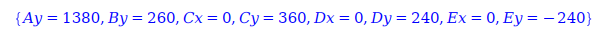
\includegraphics[width=12cm]{l9-pbq-o.png}

\section{Lecture 10}

\subsection{Lecture Question}

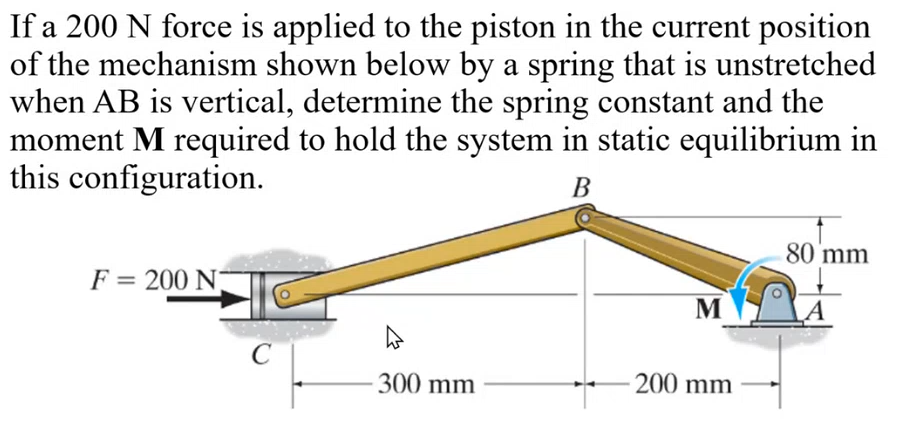
\includegraphics[width=15cm]{l10-lq.png}

We can start by finding the interior angles at A, B, and C.
Then, we can find the force of BC as well as the torque produced around A by BC.
From that, we have found the resulting moment.
Then, we can figure out how much the spring is stretched by from its natural resting position.
Using that we can find the spring constant.

Some Maple code to help with the calculations:

\begin{lstlisting}[language=matlab]
restart:
LAB:=sqrt(0.08^2 + 0.2^2): LBC:=sqrt(0.08^2 + 0.3^2):
theta:=arctan(0.08/0.2): phi:=arctan(0.08/0.3):
BC:=solve(BC*cos(phi)+200);
M:=-LAB*BC*sin(phi+theta);
sVertical:=sqrt(LBC^2-LAB^2):
stretch:=0.5 - sVertical:
k:=200/stretch;
\end{lstlisting}

The output from this code is:

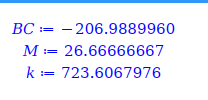
\includegraphics[width=8cm]{l10-lq-o.png}

Therefore, the moment at A is 26.6 N*m and the spring constant is 723.6 N/m.

\subsection{Lecture Quiz}

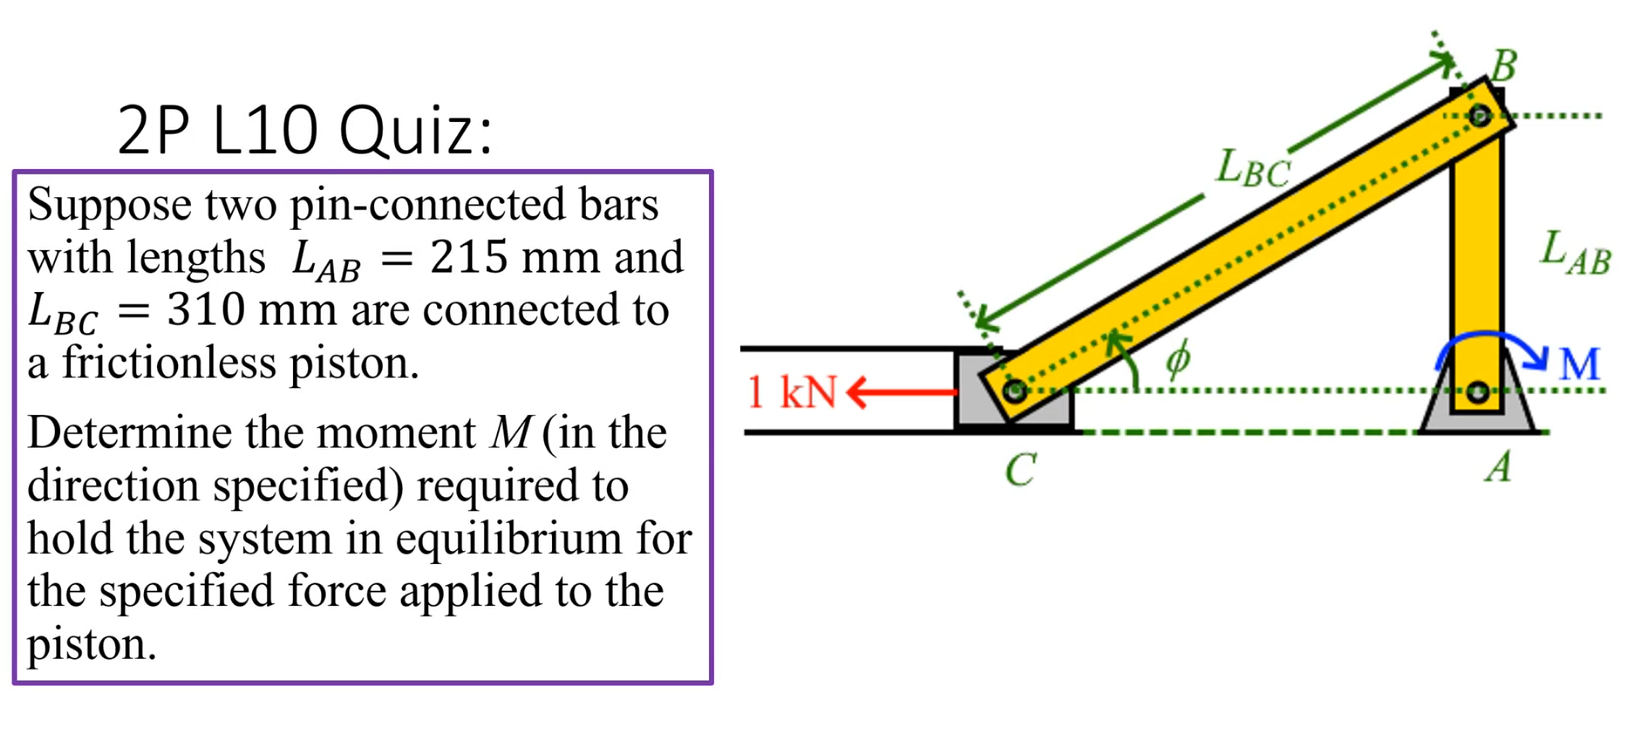
\includegraphics[width=15cm]{l10-quiz.png}

We know that there must be a reaction force and a reaction moment at A to counterraact the forces and moments from other parts of the system.
We can start by find $\phi$ which will give us the force in the BC component.
Given that, we can take the cross product of the force and the distance to find the moment at A.

Some Maple code to help with the calculations:

\begin{lstlisting}[language=matlab]
restart:
LAB:=0.215:LBC:=0.310:
phi:=arcsin(LAB/LBC):
BC:=solve(BC*cos(phi)-1000);
M:=-LAB*BC*sin(Pi/2+phi);
\end{lstlisting}

The output from this code is:

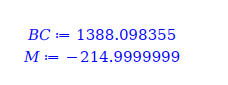
\includegraphics[width=8cm]{l10-quiz-o.png}

Therefore, the resulting moment at A is 215 N*m in the clockwise direction.

\medskip

Reflection: In this lecture, we took the concepts of frames in relation to machines and applied more complex gemoetry to them. We learned how to calculate the forces and moments in a system with more complex geometry. This is useful in real life applications where we have to deal with more complex systems. Namely, we used triangles to calculate the forces and moments in the system.

\subsection{Problem Bank Question}

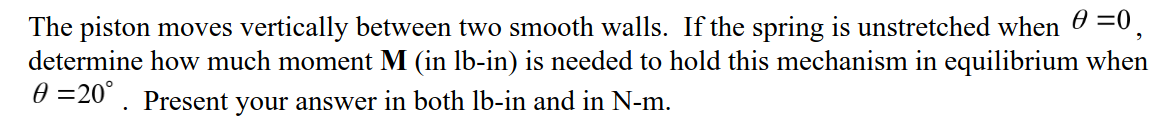
\includegraphics[width=15cm]{l10-pbq1.png}

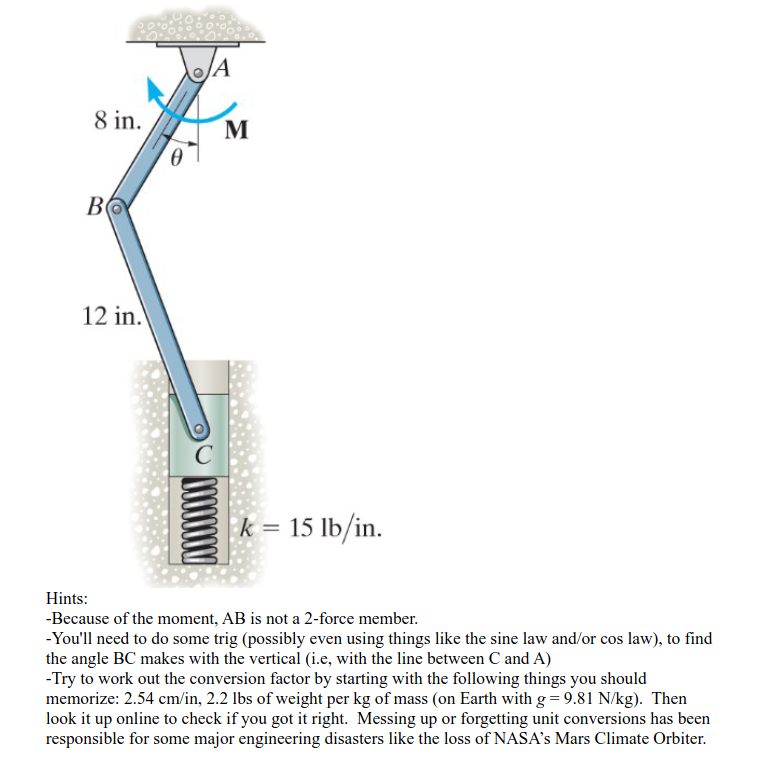
\includegraphics[width=15cm]{l10-pbq2.png}

We can start off by getting the length of the spring when it's unstretched so we can figure out it's current extension and thus force.
Then we can find the force of the spring and convert it to the force on BC.
Finally take the cross product to find the moment.

Some Maple code to help with the calculations:

\begin{lstlisting}[language=matlab]
restart:k:=15:
starting:=8+12:
# Cosine law
evalf(solve([12^2=8^2+ending^2-2*8*ending*cos(20*Pi/180), ending>0], ending)):
assign(%):
stretch:=starting-ending:
Fspring:=15*stretch;
# Sine law
solve([sin(20*Pi/180)/12 = sin(phi)/8]): assign(evalf(%)):
# Force of CB
solve([FCB*cos(phi)=Fspring]): assign(%):
tau:=-8*FCB*sin(phi+20*Pi/180);
tauMetric:=0.11298*tau;
\end{lstlisting}

The output from this code is:

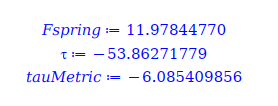
\includegraphics[width=8cm]{l10-pbq-o.png}

Therefore, the moment is -53.9 lb*in or -6.1 N*m.

\section{Lecture 11}

\subsection{Lecture Question}

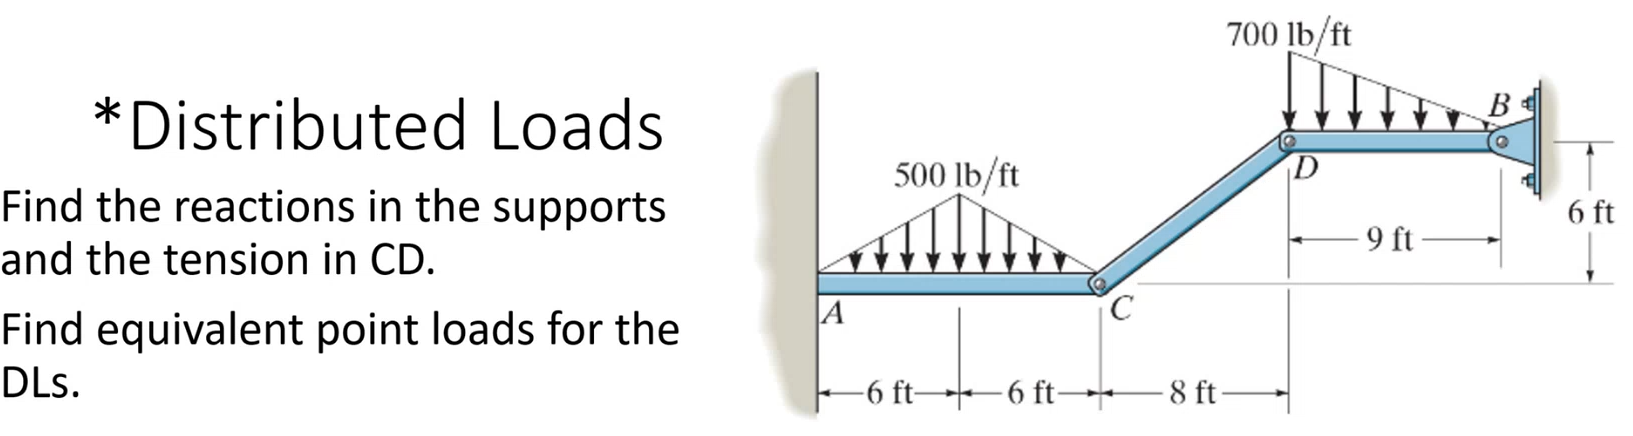
\includegraphics[width=15cm]{l11-lq.png}

We can start off by finding the force of CD from the right triangle.
We know that the x reaction force at B counterracts the force from CD, and the y reaction force at B counterracts the y component of CD plus the sum of the loaded force.
The loaded force can be found by getting the integral of the distributed load.
Since we have 3 unknowns, we can use the x and y equations as described in addition to the torque about point D.

After getting these values, we can move on and repeat this process on the left triangle to get the moment as well.

Some Maple code to help with the calculations:

\begin{lstlisting}[language=matlab]
restart:
p1:=piecewise(x<6,500*x/6, x>=6, 500*(1-(x-6)/6)):
p2:=700*(1-x/9):
tauP1A:=int(-x*pi,x=0..12):
solve([
-CD*8/sqrt(8^2+6^2) + BX,
-CD*6/sqrt(8^2+6^2) - int(p2, x=0..9) + BY,
-int(x*p2,x=0..9) + 9*BY]): assign(%):
solve([
-AX+CD*8/sqrt(8^2 + 6^2),
AY-int(p1,x=0..12)+CD*6/sqrt(8^2+6^2),
M-int(x*p1,x=0..12)+12*CD*6/sqrt(8^2+6^2)]);
\end{lstlisting}

The output from this code is:

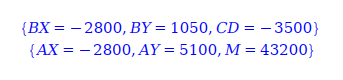
\includegraphics[width=8cm]{l11-lq-o.png}

Therefore, the force of tension in CD is 3500 lb and the moment is 43200 lb*in counterclockwise.

\subsection{Lecture Quiz}

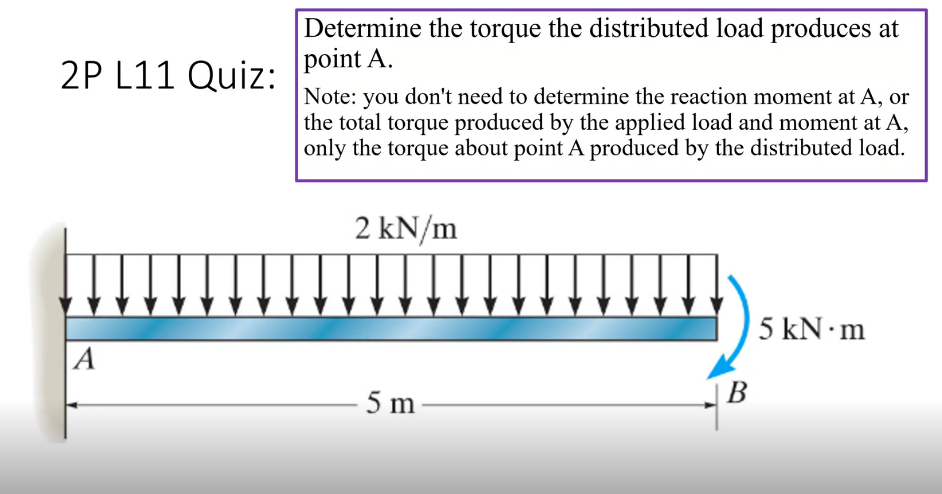
\includegraphics[width=15cm]{l11-quiz.png}

This can be solved by finding the torque from the distributed load, which we know is $\tau=\int x \cdot Fdx$.
And then we can add the 5 kN moment to that to get the total torque at point A.
We can analytically calculate the integral $\int x \cdot Fdx + 5000$ to be -25000 N*m.

\medskip

Reflection: In this lecture we learned about distributed loads and how to calculate the torque from them. This is useful in real life applications where we have to deal with distributed loads. We also learned how to calculate the torque from a moment and a distributed load.

\subsection{Problem Bank Question}

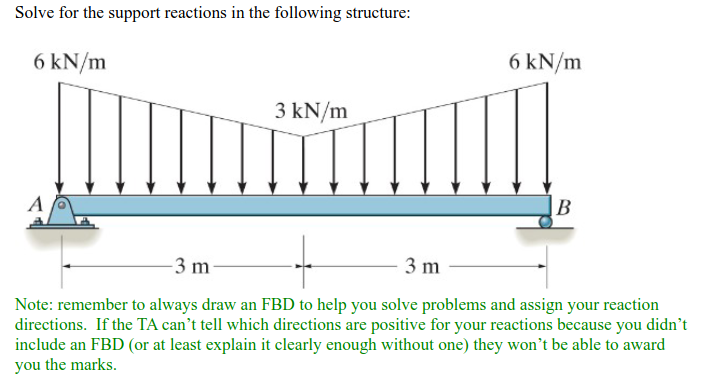
\includegraphics[width=15cm]{l11-pbq.png}

$A_x$ is positive towards the right and upwards. $B_y$ is positive upwards and no x component exists.

We can model the distributed load as a function of x and then integrate it to get the total force.
Then we can use the equations of equilibrium to solve for the unknowns.

We can use the following Maple code to help with the calculations:

\begin{lstlisting}[language=matlab]
restart: 
p:=piecewise(x<3,6-x,x>=3,x);
force:=int(p,x=0..6);
tau:=int(x*p,x=0..6);
solve([
Ay+By-force,
Ax,
-tau+6*By]): evalf(%);
\end{lstlisting}

The output from this code is:

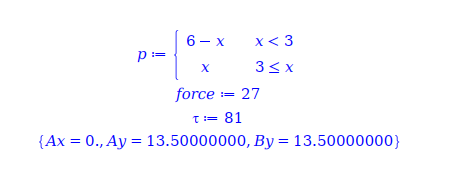
\includegraphics[width=8cm]{l11-pbq-o.png}

Therefore, the x component of A is 0, and the y components of both A and B are 13.5 kN upwards.

\end{document}
